\section{Remaking GIRAF prototypes}\label{prototype-comp}
We inherited a set of PowerPoint slides from last year's product owner group, as described in \autoref{prepared-work-from-previous-years}.
The different functionalities of the prototypes will be explained in the following section.
The most relevant updated prototypes will also be compared to the previous versions.

\subsection{The functionalities of the prototypes}
As we decided to make new prototypes, it was essential that we fulfilled all the necessary functionalities determined by the previous year in conjunction with the customers.
From reading the reports of the previous year and looking at the inherited prototypes we defined the following list of functionalities to design prototypes for:
\begin{itemize}
    \item Login functionality
    \item Select a citizen to view the week plans
    \item Add a week plan to a citizen
    \item View an actual week plan
    \item Add activities to a week plan
    \item Mark activities in the week plan
    \item Add timers to activities
    \item View and change settings
\end{itemize}
Designing the necessary prototypes left us with a total of around 65 different prototypes of different screens of the GIRAF weekplanner application.

\subsection{Comparisons of old and new prototypes}
The following section presents and compares a subset of the new and old prototypes. 

\subsubsection{The login and choosing citizen screens}
The base design of the previous login screen was functionally acceptable. 
The background colour used was just a dull yellow, and as such we decided to update the background to be a little more dynamic but keeping the separate bars in which to input \texttt{username} and \texttt{password}.
The design change used for logging in was also employed in the confirmation screen from swapping from citizen to guardian mode. 
\begin{figure}[H]
    \begin{subfigure}{0.5\textwidth}
    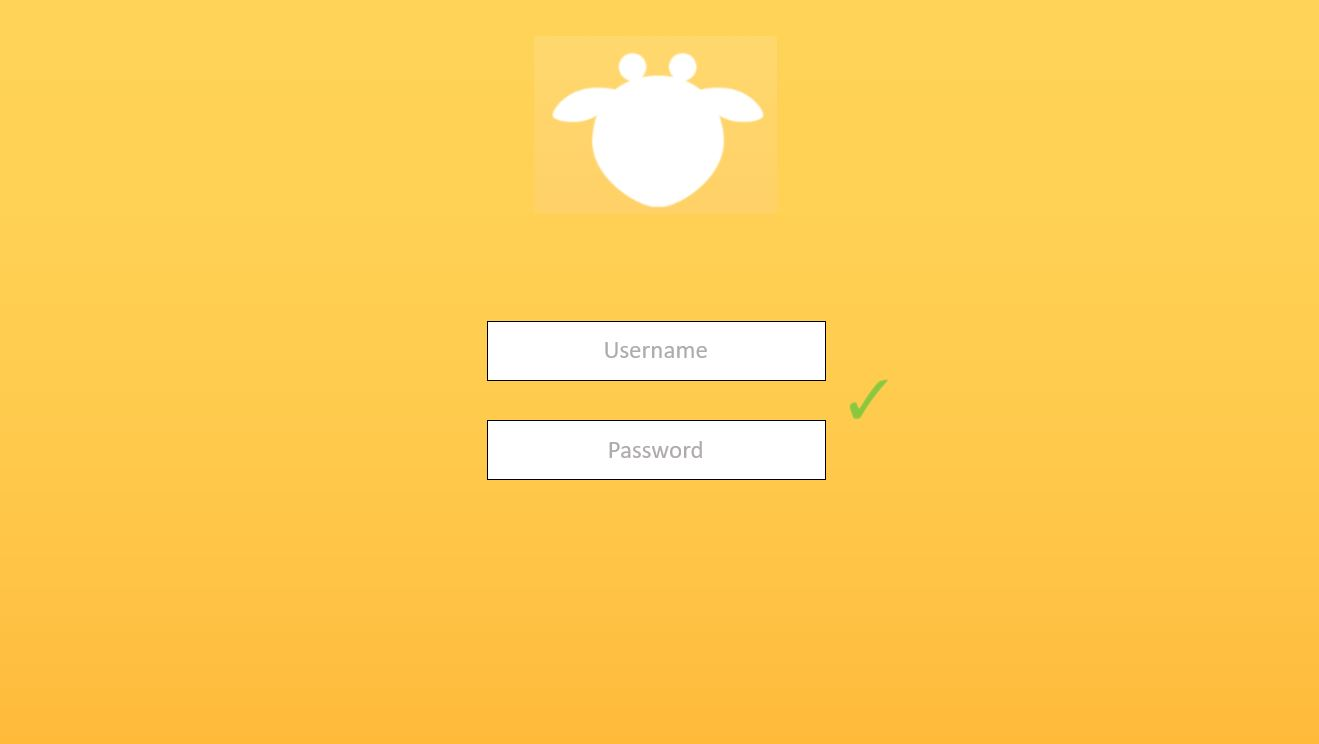
\includegraphics[width=1\linewidth, height=5cm]{old_login.JPG} 
    \caption{The previous login screen}
    \label{fig:previous_login}
    \end{subfigure}
    \begin{subfigure}{0.5\textwidth}
        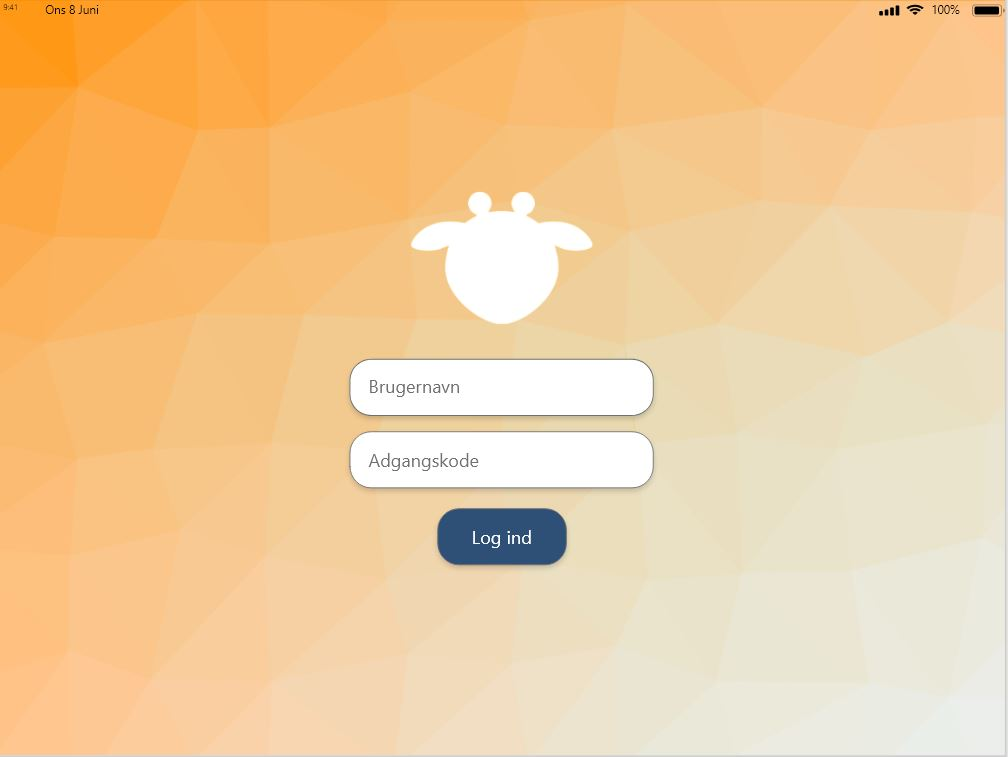
\includegraphics[width=1\linewidth, height=5cm]{new_login.JPG}
    \caption{The proposed new login screen}
    \label{fig:new_login}
    \end{subfigure} 
    \caption{This figure shows both designs for the login screen.}
    \label{fig:guardian_confirm}
\end{figure}
\noindent
\begin{figure}[H]
    \begin{subfigure}{0.5\textwidth}
    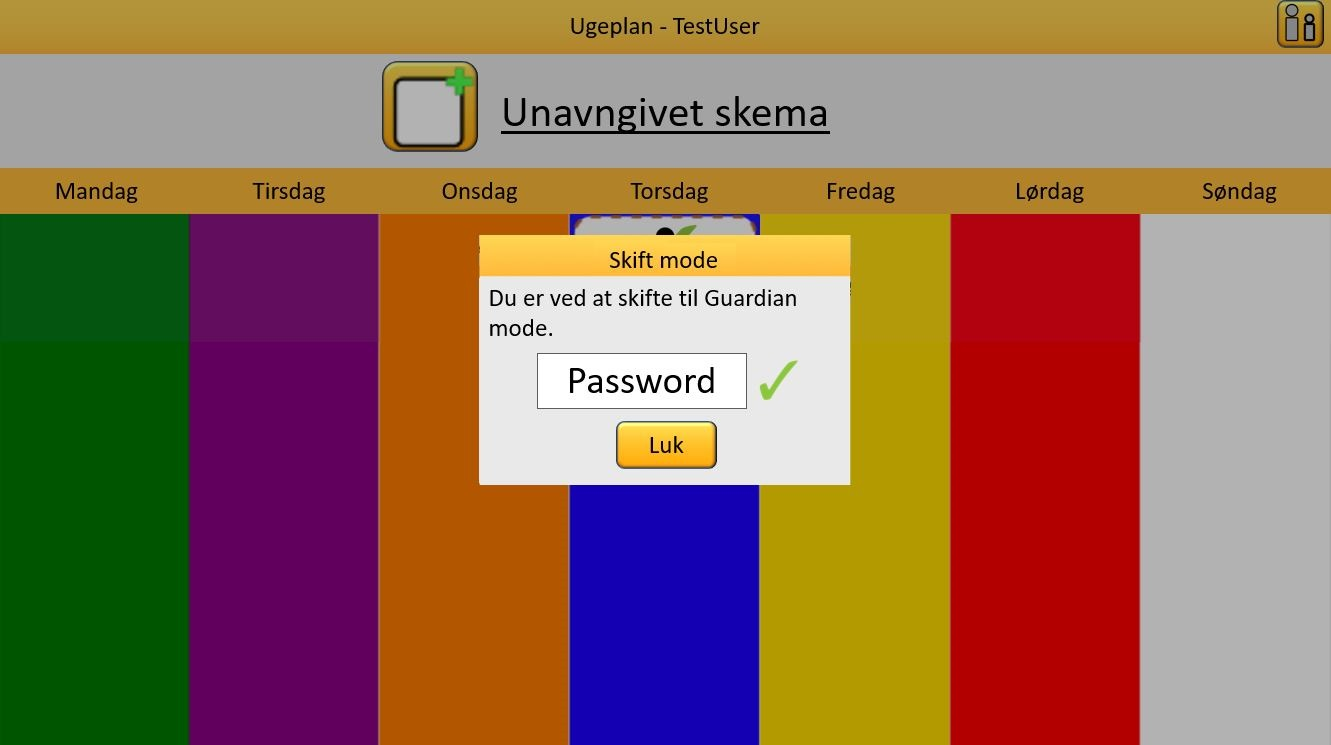
\includegraphics[width=1\linewidth, height=5cm]{previous_password_change.JPG} 
    \caption{The previous confirmation}
    \label{fig:previous_guardian_confirm}
    \end{subfigure}
    \begin{subfigure}{0.5\textwidth}
        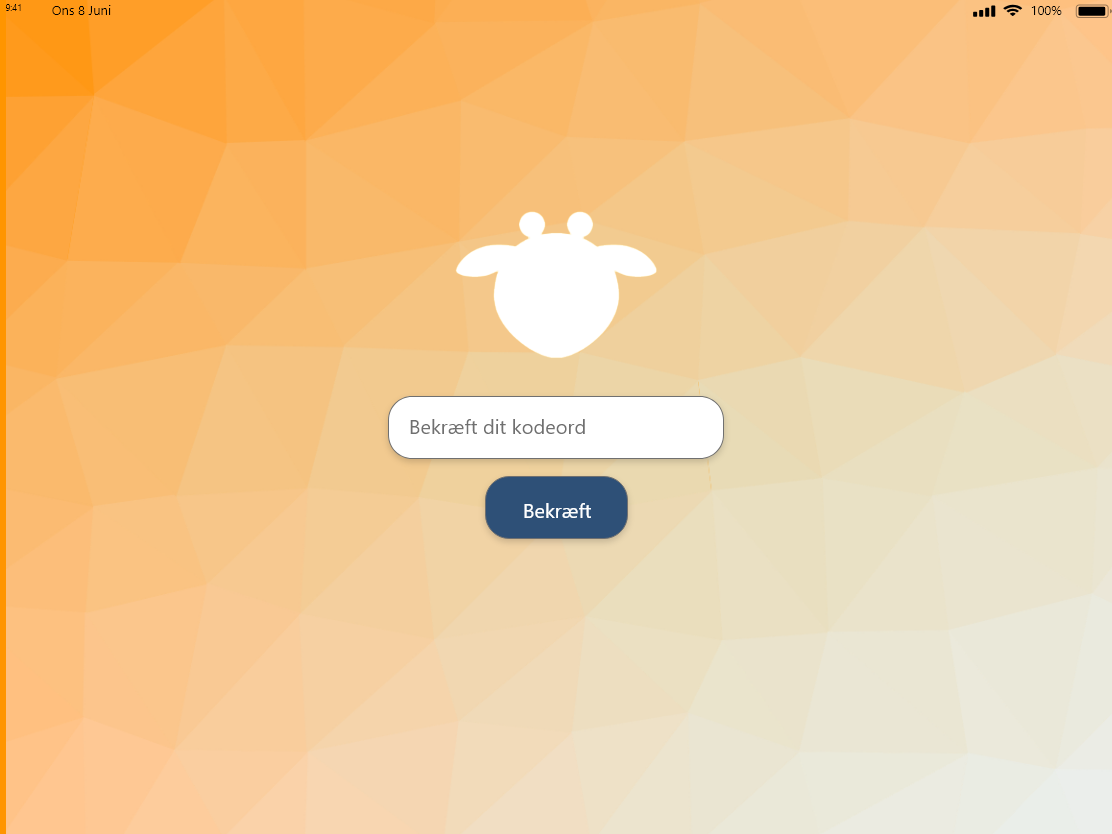
\includegraphics[width=1\linewidth, height=5cm]{guardian_switch_confirm.png}
    \caption{The proposed new change screen}
    \label{fig:new_guardian_confirm}
    \end{subfigure} 
    \caption{This figure shows both designs for confirming password when changing from citizen to guardian.}
    \label{fig:guardian_confirm_comparison}
\end{figure}
\noindent
The design of the screen where citizens are selected was also changed.
It was  primarily changed to make it more aesthetically pleasing, with the main selection area being changed to a scrollable window with two columns. 
\begin{figure}[H]
    \begin{subfigure}{0.5\textwidth}
    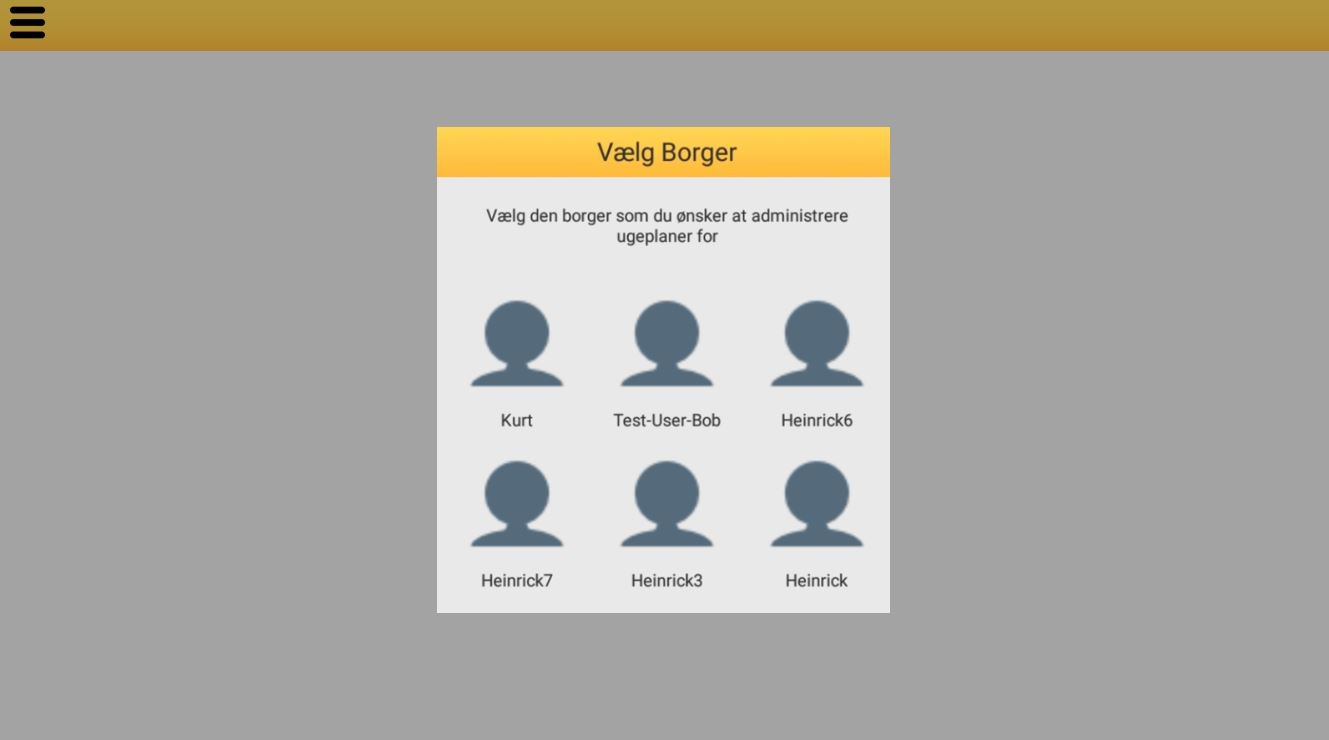
\includegraphics[width=1\linewidth, height=5cm]{previous_citizen_select.JPG} 
    \caption{The previous citizen selection}
    \label{fig:previous_citizen_select}
    \end{subfigure}
    \begin{subfigure}{0.5\textwidth}
        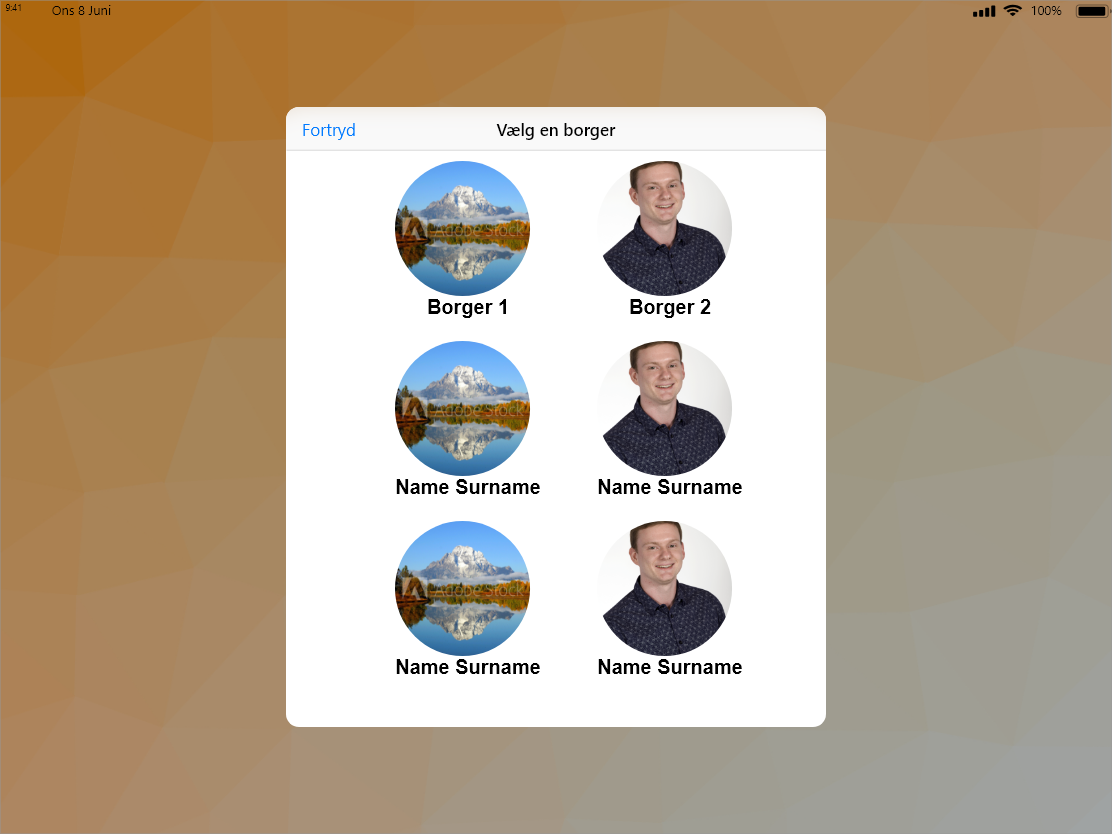
\includegraphics[width=1\linewidth, height=5cm]{copy_weekplan_choose_citizen.png}
    \caption{The proposed new citizen selection}
    \label{fig:new_citizen_select}
    \end{subfigure} 
    \caption{This figure shows both designs for choosing a citizen to view their week plans.}
    \label{fig:citizen_select}
\end{figure}
\noindent

\subsubsection{The overall week plan view}
The main changes made in the overall view of the week plan was the design. 
The top bar was changed to include new icons, and the generic phone/tablet bar was added to let the user keep an overview of the status of their device.
We removed the large area reserved for the name of the week plan on the previous suggestions, to give more space for the week plan to be used. 
\begin{figure}[H]
    \begin{subfigure}{0.5\textwidth}
    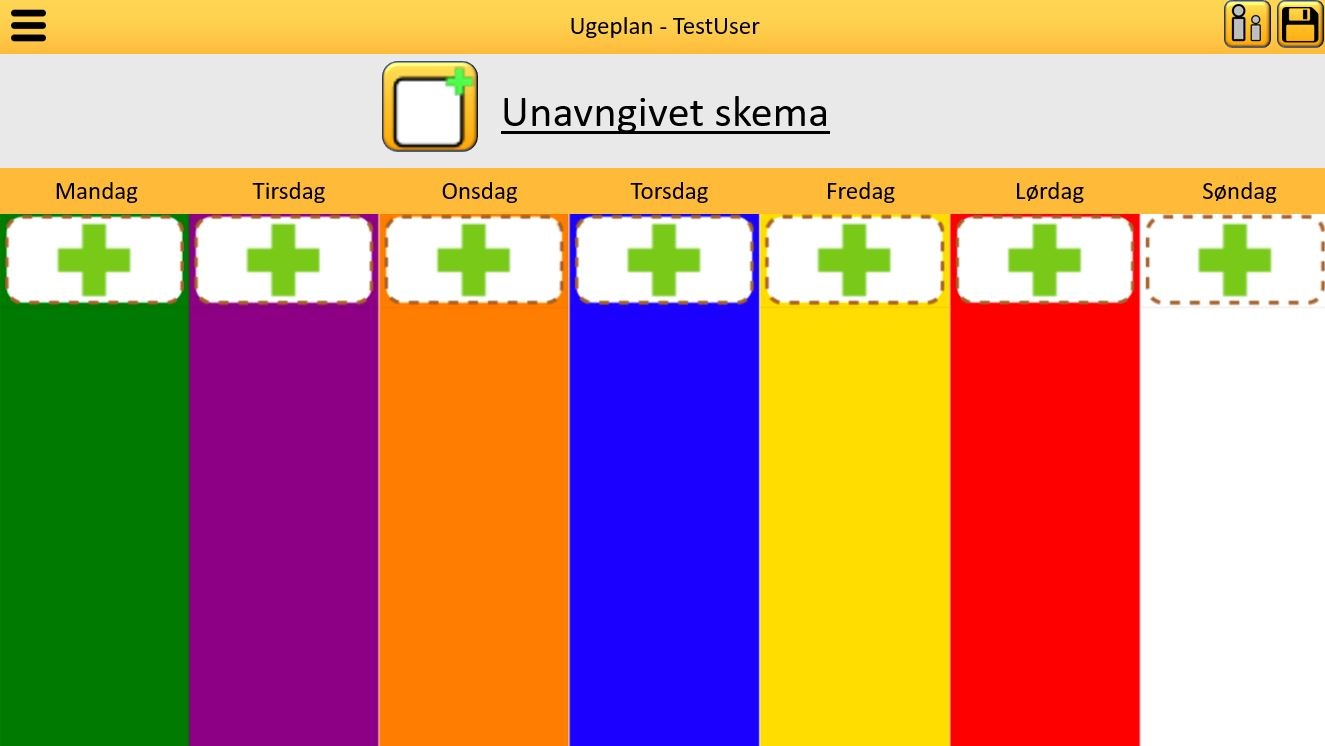
\includegraphics[width=1\linewidth, height=5cm]{previous_ugeplan.JPG} 
    \caption{The previous week plan view}
    \label{fig:previous_weekplan_view}
    \end{subfigure}
    \begin{subfigure}{0.5\textwidth}
        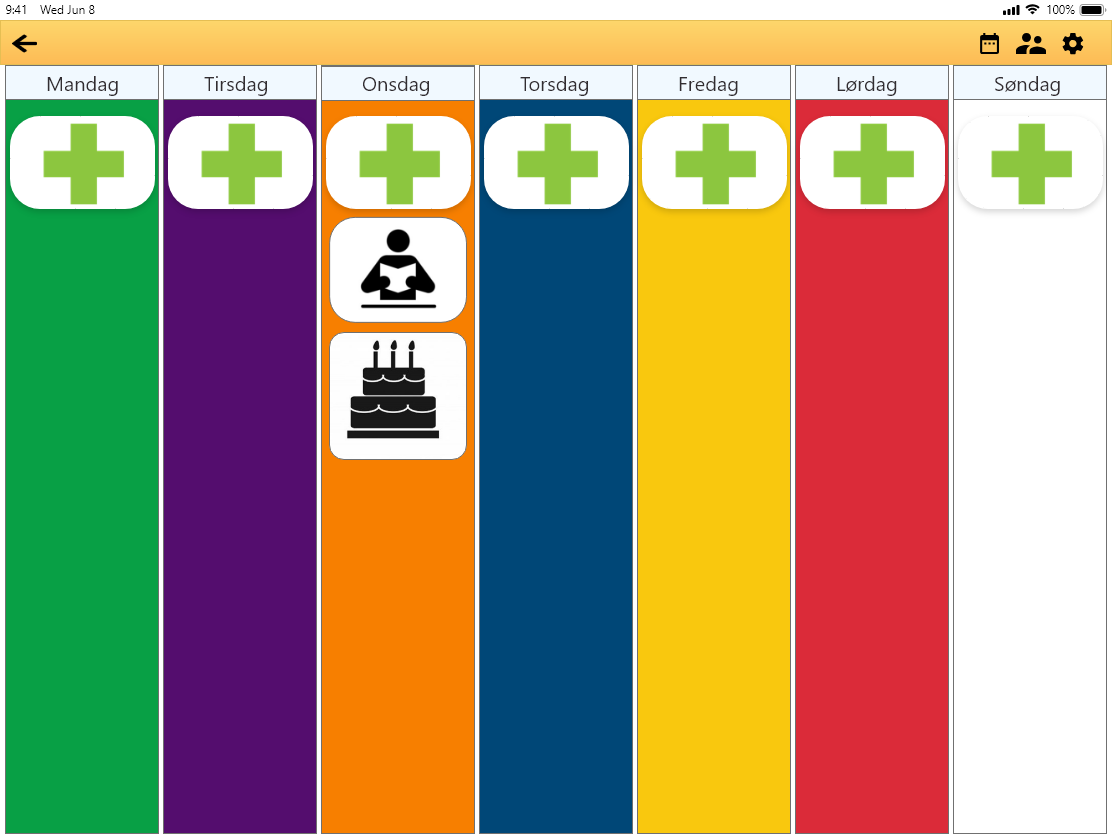
\includegraphics[width=1\linewidth, height=5cm]{ugeplan_guardian_view.png}
    \caption{The proposed new week plan view}
    \label{fig:new_weekplan_view}
    \end{subfigure} 
    \caption{This figure shows both designs for the week plan from a guardian point of view.}
    \label{fig:weekplan_view}
\end{figure}

\subsubsection{Mark mode functionality}
In order to improve usability the weekplanner should support functionality to perform actions on multiple activities at the same time.
The previous prototypes featured a retractable side menu that the new prototypes do not.
As such, the main difference was in how \textit{mark mode} was activated. 
On the new prototypes we implemented a symbol on the top bar to activate this functionality.
\begin{figure}[H]
    \begin{subfigure}{0.5\textwidth}
    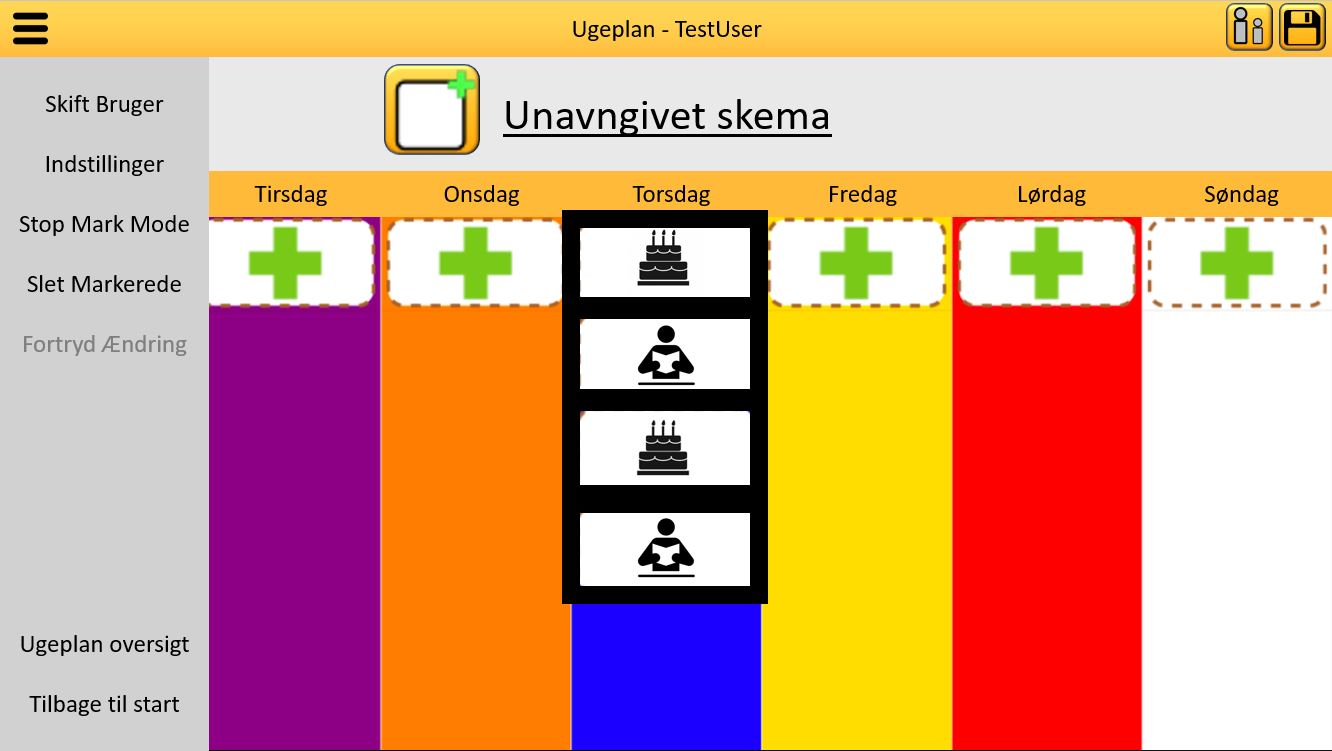
\includegraphics[width=1\linewidth, height=5cm]{old_markmode.JPG} 
    \caption{The previous mark mode functionality}
    \label{fig:old_markmode}
    \end{subfigure}
    \begin{subfigure}{0.5\textwidth}
        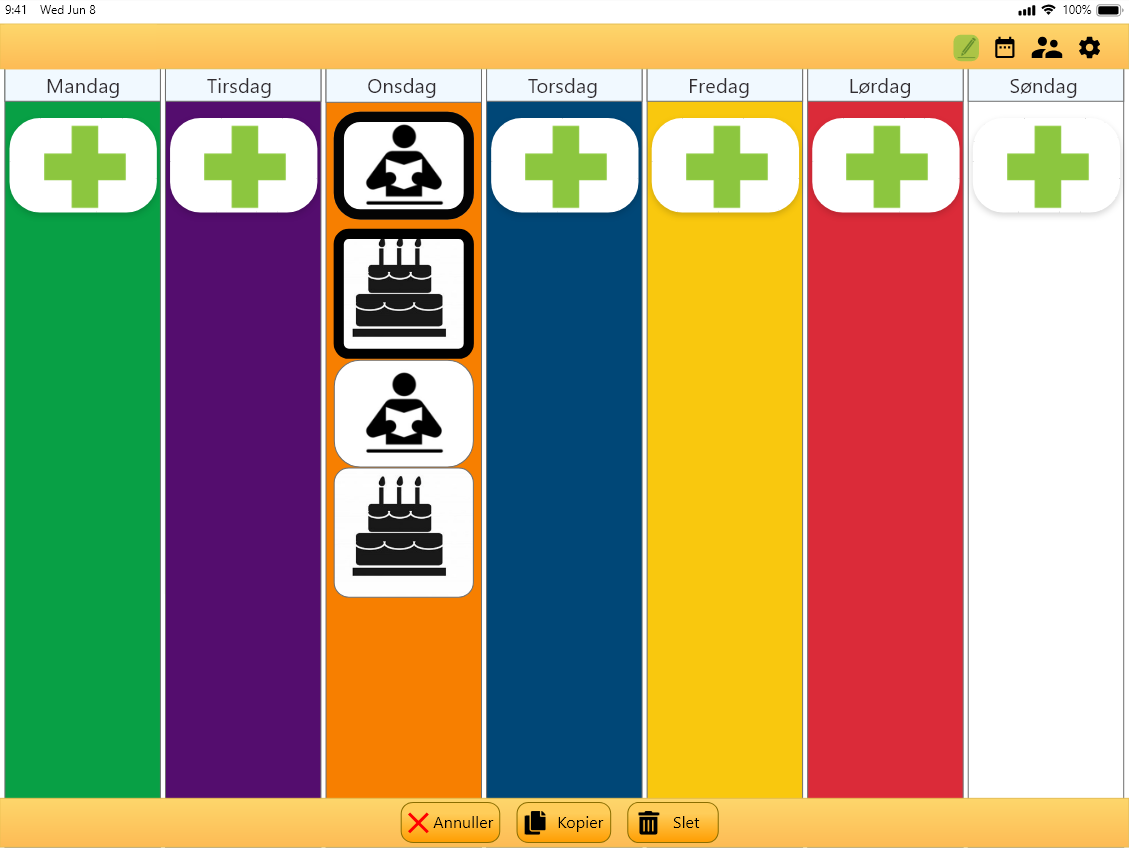
\includegraphics[width=1\linewidth, height=5cm]{new_markmode.PNG}
    \caption{The proposed new way to use mark mode}
    \label{fig:new_markmode}
    \end{subfigure} 
    \caption{This figure shows the different mark mode prototypes.}
    \label{fig:markmode_prototypes}
\end{figure}

\subsubsection{Details for an activity}
Users should be able to look at the details of an activity.
When they do this, they should be able to add a timer or change the status of the activity.
We kept the structure of the previous prototype, but redid the design for this to include less text. 
This was done since the customers expressed an interest in as little text as possible.
\begin{figure}[H]
    \begin{subfigure}{0.5\textwidth}
    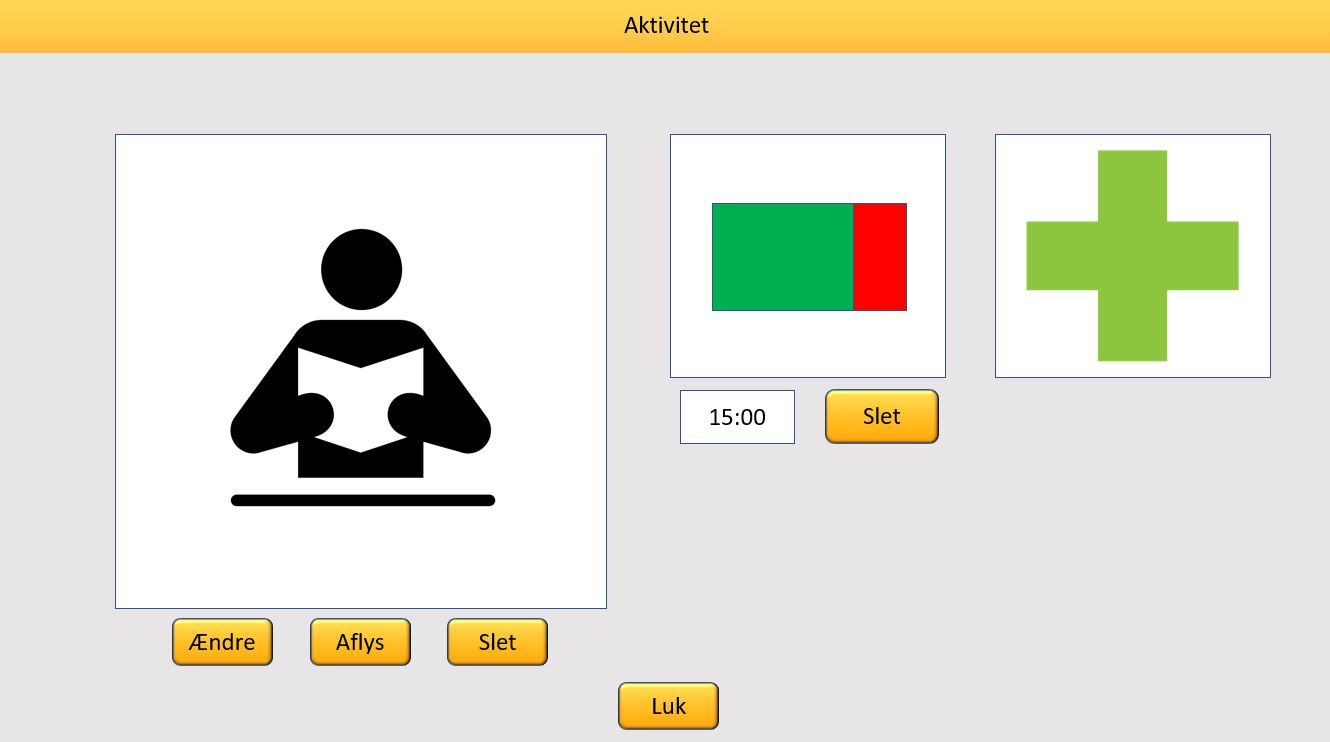
\includegraphics[width=1\linewidth, height=5cm]{old_activity_detail.JPG} 
    \caption{The previous detail prototype}
    \label{fig:old_activity_detail}
    \end{subfigure}
    \begin{subfigure}{0.5\textwidth}
        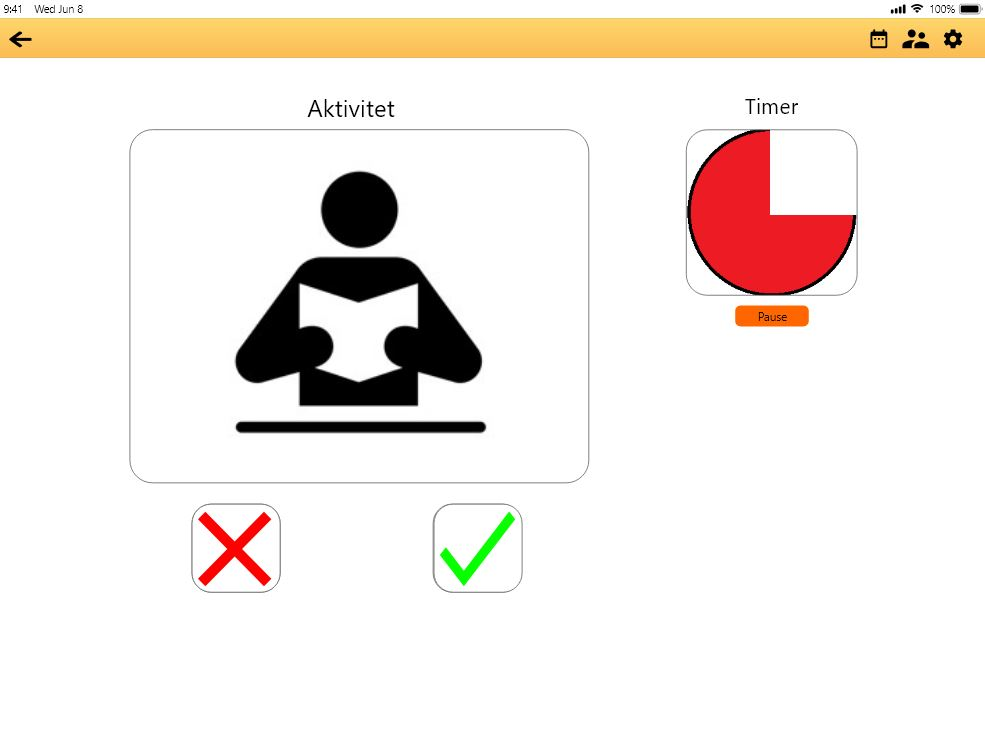
\includegraphics[width=1\linewidth, height=5cm]{new_activity_detail.JPG}
    \caption{The new detail prototype}
    \label{fig:new_activity_details}
    \end{subfigure} 
    \caption{This figure shows the screens for activity details.}
    \label{fig:activity_detail_prototypes}
\end{figure}
